% -*- coding: latin-1 -*-
\section{Pitch-detection}
RT\_LPC giver mulighed for at detektere pitch vha. autokorrelation. Vi har dog istedet implementeret average magnitude difference (AMDF) pitch detection p� baggrund af [Sayood] pp. 543. Formlen for AMDF er:

\begin{equation}
AMDF(p) = \frac{1}{N} \sum^{N-1}_{i=0}\left|y_i-y_{(i+p) \% N}\right|
\end{equation}

hvor p er perioden. 

Vi benytter v�rdier af $p$ som giver mening for menneskelig tale, hvor den l�ngste periode er 19,5 ms og den korteste er 2,5 ms. 
Det giver dog ikke mening at detektere perioder, der er kortere end den stump signal man arbejder med, s� vi v�lger den l�ngste periode til 70\% af vinduest�rrelsen. V�rdier herover giver undertoner pr�get af vinduest�rrelsen, s�ledes at en 20 ms buffer eksempelvis giver en 50 Hz undertone.

\subsection{Stemte lyde}
I f�lgende eksempel analyseres 20 ms af 'y'-lyden i 'tydelig'.

\begin{figure}
\begin{center}
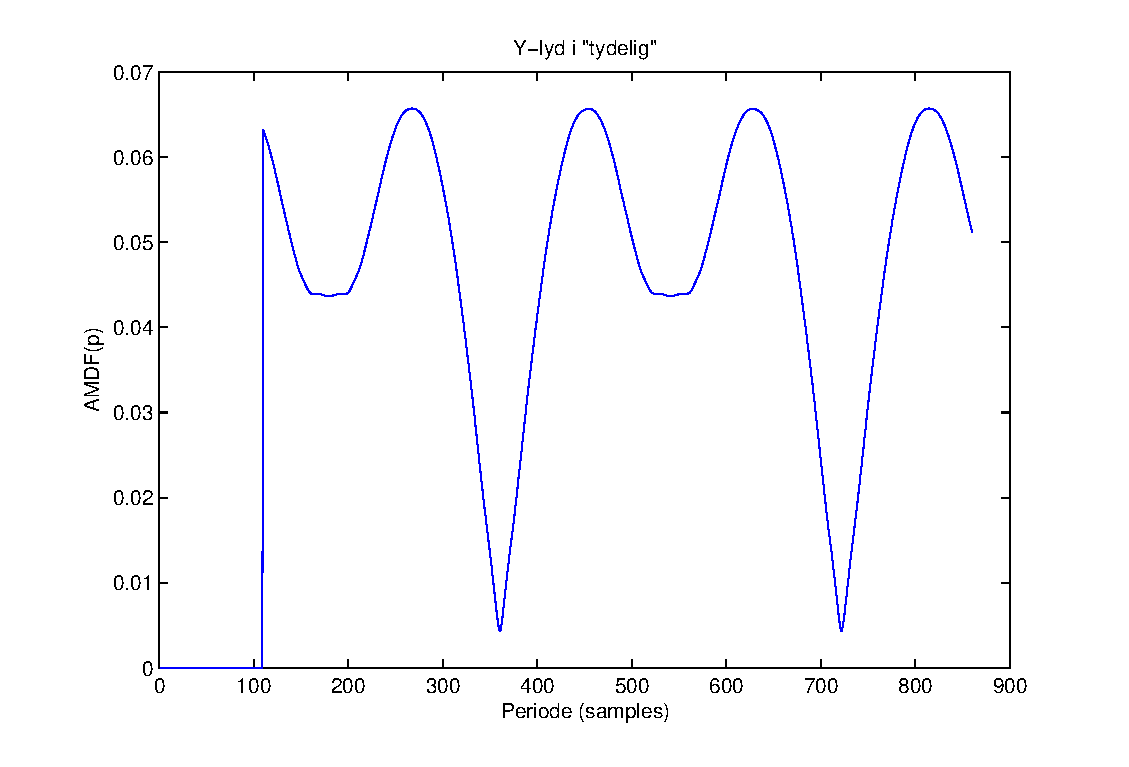
\includegraphics[width=120mm]{y-plot.eps}\\
\end{center}
\label{udstyr}
\caption{'Y'-lyd i 'tydelig'}
\end{figure}

Det ses at minimum ligger ved ca 730 samples, svarende til ca 60 Hz. Et lokalt minimum ses ved den dobbelte frekvens (den halve periode), hvilket formodentligt er en overtone.

\subsection{Ustemte lyde}
Er den minimale v�rdi over et bestemt threshold, v�lger vi at opfatte frame'n som en ustemt lyd.

I dette ekspempel analyseres 20 ms af 't'-lyden i 'tydelig'. Det ses at alle v�rdier ligger forholdsvist samme sted p� y-aksen. Ingen v�rdi er under vores threshold og vi opfatter derfor frame'n som en ustemt lyd.

\begin{figure}
\begin{center}
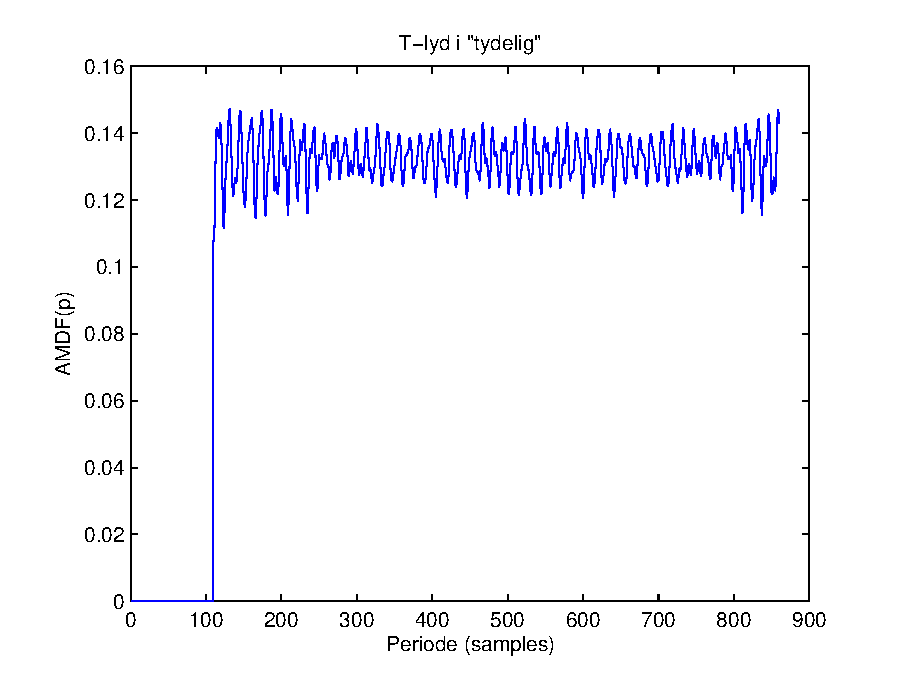
\includegraphics[width=120mm]{t-plot.eps}\\
\end{center}
\label{udstyr}
\caption{'T'-lyd i 'tydelig'}
\end{figure}

